% ===================================
% CODICE LaTeX PER GRAFICI E TABELLE
% Tesi GDO - Capitoli 1 e 2
% ===================================
% filepath: c:\Users\saint\tesi\nuovi grafi 1 e 2.tex
\documentclass[border=10pt]{standalone}
% Pacchetti necessari
\usepackage[utf8]{inputenc}
\usepackage[T1]{fontenc}
\usepackage{amsmath}
\usepackage{amssymb}    
\usepackage{graphicx}
\usepackage{caption}
\usepackage{subcaption} % Per sottotitoli nelle figure
% Preambolo necessario:
\usepackage{tikz}
\usepackage{pgfplots}
\usepackage{booktabs}
\usepackage{multirow}
\pgfplotsset{compat=1.17}
\usetikzlibrary{pgfplots.polar}

% ===================================
% CAPITOLO 1
% ===================================
% FIGURA 1.2: Framework GIST - Architettura Concettuale
\begin{document}
\centering
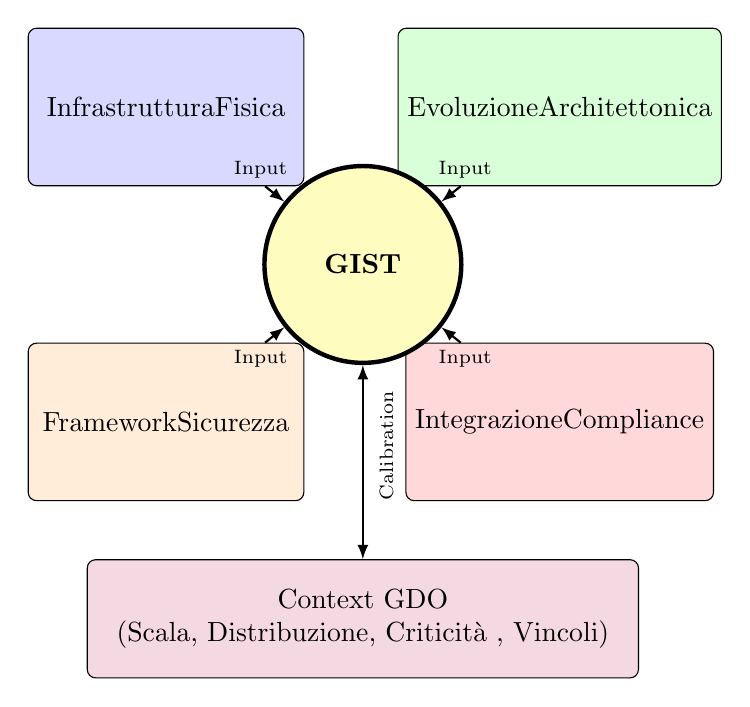
\begin{tikzpicture}[
    box/.style={rectangle, draw, text centered, minimum width=3.5cm, minimum height=2cm, rounded corners=3pt},
    contextbox/.style={rectangle, draw, text centered, minimum width=7cm, minimum height=1.5cm, rounded corners=3pt},
    arrow/.style={->, thick, >=latex},
    node distance=3.5cm
]

% Componenti principali
\node[box, fill=blue!15] (physical) at (0,0) {Infrastruttura\newline Fisica};
\node[box, fill=green!15] (arch) at (5,0) {Evoluzione\newline Architettonica};
\node[box, fill=orange!15] (security) at (0,-4) {Framework\newline Sicurezza};
\node[box, fill=red!15] (compliance) at (5,-4) {Integrazione\newline Compliance};

% Framework centrale GIST
\node[circle, draw, fill=yellow!25, minimum size=2.5cm, ultra thick] (gist) at (2.5,-2) {\textbf{GIST}};

% Context GDO
\node[contextbox, fill=purple!15, align=center] (context) at (2.5,-6.5) {Context GDO\\(Scala, Distribuzione, Criticità , Vincoli)};

% Connessioni
\draw[arrow] (physical) -- (gist);
\draw[arrow] (arch) -- (gist);
\draw[arrow] (security) -- (gist);
\draw[arrow] (compliance) -- (gist);
\draw[arrow, <->] (gist) -- (context);

% Etichette delle connessioni
\node[font=\scriptsize] at (1.2,-0.8) {Input};
\node[font=\scriptsize] at (3.8,-0.8) {Input};
\node[font=\scriptsize] at (1.2,-3.2) {Input};
\node[font=\scriptsize] at (3.8,-3.2) {Input};
\node[font=\scriptsize, rotate=90] at (2.8,-4.3) {Calibration};
\end{tikzpicture}
\end{document}
